\documentclass[10pt,a4paper]{article}
\newtheorem{theorem}{Theorem} 
\newtheorem{lemma}{Lemma} 
\newtheorem{proposition}{Proposition} 
\newtheorem{proof}{Proof} 
\newtheorem{definition}{Definition}
\usepackage[latin1]{inputenc}
\usepackage[T1]{fontenc}
\usepackage{amsmath}
\usepackage{amsfonts}
\usepackage{amssymb}
\usepackage{makeidx}
\usepackage{graphicx}
\usepackage{float}
\usepackage{ifpdf}
\ifpdf
\usepackage[breaklinks,hidelinks]{hyperref}
\else 
\usepackage{url}
\fi
\author{student}
\title{Scratch Pad Fuzzy Set}
\begin{document}
\maketitle

\noindent sympy.stats.Normal(name, mean, std) \\ Create a continuous random variable with a Normal distribution. \\ The density of the Normal distribution is given by 
\begin{equation}
\begin{minipage}{300pt}
 $\displaystyle f{\left (x \right )} = \frac{\sqrt{2} e^{- \frac{\left(\mu - x\right)^{2}}{2 \sigma^{2}}}}{2 \sqrt{\pi} \sigma}$  
\end{minipage}
\end{equation}
\noindent Parameters:	\\ mu    : Real number or a list representing the mean or the mean vector \\ sigma : Real number or a positive definite sqaure matrix, \\ $\sigma^{2} > 0 $ the variance \\ Returns: A Random Symbol.  \\ \\ References  \\ $[R575]$	\url{http://en.wikipedia.org/wiki/Normal_distribution}  \\ $[R576]$	\url{http://mathworld.wolfram.com/NormalDistributionFunction.html}
\noindent The sympy function 
\begin{equation}
\begin{minipage}{300pt}
 $\displaystyle f_{1} = NormalDistribution(\mu, \sigma)$  
\end{minipage}
\end{equation}
\noindent declares the Normal Distribution 
\noindent The following function specifies the random variable $z$
\begin{equation}
\begin{minipage}{300pt}
 $\displaystyle f_{2} = \operatorname{f_{1}}{\left (z \right )} = \frac{\sqrt{2}}{2 \sqrt{\pi} \sigma} e^{- \frac{\left(- \mu + z\right)^{2}}{2 \sigma^{2}}}$  
\end{minipage}
\end{equation}
\begin{equation}
\begin{minipage}{300pt}
 $\displaystyle f_{3} = \int_{z_{i}}^{z_{f}} \operatorname{f_{2}}{\left (z \right )}\, dz = \frac{1}{2} \operatorname{erf}{\left (\frac{\sqrt{2}}{2 \sigma} \left(- \mu + z_{f}\right) \right )} - \frac{1}{2} \operatorname{erf}{\left (\frac{\sqrt{2}}{2 \sigma} \left(- \mu + z_{i}\right) \right )}$  
\end{minipage}
\end{equation}
\noindent Let $\mu = 0 $ and $\sigma = 1 $ then 
\begin{equation}
\begin{minipage}{300pt}
 $\displaystyle f_{3} = \int_{-\infty}^{\infty} \operatorname{f_{2}}{\left (z \right )}\, dz = 1$  
\end{minipage}
\end{equation}
\begin{equation}
\begin{minipage}{300pt}
 $\displaystyle \int_{-1}^{1} \operatorname{f_{2}}{\left (z \right )}\, dz = \operatorname{erf}{\left (\frac{\sqrt{2}}{2} \right )} = 0.682689492137086$  
\end{minipage}
\end{equation}
\begin{equation}
\begin{minipage}{300pt}
 $\displaystyle \int_{-3}^{3} \operatorname{f_{2}}{\left (z \right )}\, dz = \operatorname{erf}{\left (\frac{3 \sqrt{2}}{2} \right )} = 0.99730020393674$  
\end{minipage}
\end{equation}
\begin{equation}
\begin{minipage}{300pt}
 $\displaystyle \int_{-6}^{6} \operatorname{f_{2}}{\left (z \right )}\, dz = \operatorname{erf}{\left (3 \sqrt{2} \right )} = 0.999999998026825$  
\end{minipage}
\end{equation}
\begin{equation}
\begin{minipage}{300pt}
 $\displaystyle DPM = 317310.507862914$  
\end{minipage}
\end{equation}
\begin{equation}
\begin{minipage}{300pt}
 $\displaystyle DPM = 2699.79606326021$  
\end{minipage}
\end{equation}
\begin{equation}
\begin{minipage}{300pt}
 $\displaystyle DPM = 0.00197317528982666$  
\end{minipage}
\end{equation}
\noindent A set of values of $z$ can be generated randomly by the sympy function \\     $Normal(\mu, \sigma)$. Given  $\mu = 5 $ and $\sigma = 0.5 $ then 
\begin{equation}
\begin{minipage}{300pt}
 $\displaystyle f_{1} = NormalDistribution(5, 0.5)$  
\end{minipage}
\end{equation}
\begin{equation}
\begin{minipage}{300pt}
 $\displaystyle f_{2} = \frac{1.0 \sqrt{2}}{\sqrt{\pi}} e^{- 2.0 \left(z - 5\right)^{2}}$  
\end{minipage}
\end{equation}
\begin{equation}
\begin{minipage}{300pt}
 $\displaystyle f_{3} = \int_{z_{i}}^{z_{f}} \operatorname{f_{2}}{\left (z \right )}\, dz = \\ 0.353553390593274 \sqrt{2} \operatorname{erf}{\left (1.4142135623731 z_{f} - 7.07106781186548 \right )} - 0.353553390593274 \sqrt{2} \operatorname{erf}{\left (1.4142135623731 z_{i} - 7.07106781186548 \right )}$  
\end{minipage}
\end{equation}
\noindent \section{Material}  A set of values of $z$ can be generated     randomly by the sympy function \\ $Normal(\mu, \sigma)$. Given  $\mu = 5 $ and $\sigma = 0.5 $ then for 10000 pieces we have \\ \\ 
\begin{equation}
\begin{minipage}{300pt}
 $\displaystyle Rods = random.normal(nmu, nsigma, count) = [10.39764384  9.72348858  9.10724766 ... 10.19747606  9.96031815
 10.33428485]$  
\end{minipage}
\end{equation}
\noindent The histogram of (15) is shown in Figure 1.
\begin{figure}[H]
\centering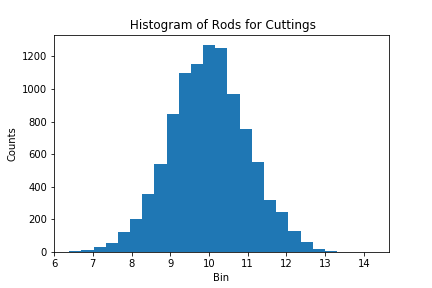
\includegraphics[width=1\linewidth,height=0.25\textheight]{Fig01}
\caption{Histogram Rods Variation}
\label{fig:Fig01}
\end{figure}

\noindent Given the specification of $\pm 1$, how many are good and what is the    yield? 
\noindent Answer number of good rods = 9528, yield = 95.28\%. Note that everytime the program is run these    values changes. The solution used is to use an algorithm to check each    rod and count those that are within tolerance. Try solving it using (14)    and compare the results. \\ \\ \section{Equipment}    Now consider that these rods are to be cut into    halves. The cutter has $\mu = 0.5 $ and $\sigma = 0.05 $ then for 9528 pieces we have \\ \\ 
\begin{equation}
\begin{minipage}{300pt}
 $\displaystyle f_{1} = NormalDistribution(0.5, 0.05)$  
\end{minipage}
\end{equation}
\begin{equation}
\begin{minipage}{300pt}
 $\displaystyle f_{2} = \frac{10.0 \sqrt{2}}{\sqrt{\pi}} e^{- 200.0 \left(z - 0.5\right)^{2}}$  
\end{minipage}
\end{equation}
\begin{equation}
\begin{minipage}{300pt}
 $\displaystyle f_{3} = \int_{z_{i}}^{z_{f}} \operatorname{f_{2}}{\left (z \right )}\, dz = \\ 0.353553390593274 \sqrt{2} \operatorname{erf}{\left (14.1421356237309 z - 7.07106781186547 \right )}$  
\end{minipage}
\end{equation}
\begin{equation}
\begin{minipage}{300pt}
 $\displaystyle Cut_{event} = random.normal(nmu, nsigma, len(GoodRod)) = [0.54263729 0.48660446 0.48125061 ... 0.46560666 0.50735312 0.51214978]$  
\end{minipage}
\end{equation}
\noindent The histogram of (19) is shown in Figure 2.
\begin{figure}[H]
\centering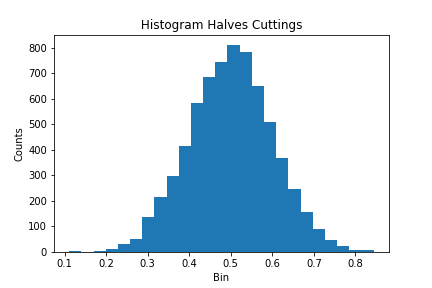
\includegraphics[width=1\linewidth,height=0.25\textheight]{Fig02}
\caption{Histogram of Cutter Variation}
\label{fig:Fig02}
\end{figure}

\noindent \section{Method}    There two methods to cut the rod. One method is the cutter is place at  a    distance of half the rod size exactly 5. Then the rod is referenced at the    point of origin and cut is made.  The other method is to place the rod    at its center for cutter engagement. The formulas for the two methods are    different. Determine the formula for each and justify it.
\noindent \\ \\ Answers: \\ 1. The cutter with variation, i.e., $5 \pm .25$  is    multiplied by the perfect dimension of rod that is 10. Then the answer is    substracted from rod with variation. The two answer are the cut products.    \\ 2. The rod with variation, i.e., $ 10 \pm 1$ is multiplied by the    cutter with variation, i.e., $5 \pm .25$. The answer is substracted from    the rod with variation. The cut producst are the two answers. \\ \\    Determine the average and standard deviation of cut rods for each method    and compare them. What is your observation?
\noindent The histograms of Method 1 and 2 are shown in Figure 3.
\begin{figure}[H]
\centering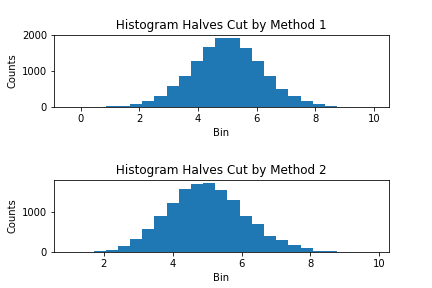
\includegraphics[width=1\linewidth,height=0.5\textheight]{Fig03}
\caption{Histogram of Cut Rods}
\label{fig:Fig03}
\end{figure}

\noindent Assuming that the cut specification is $5 \pm .5$, determine the number    of good cut and the yield for each method
\noindent The number of good cut for method 1 is $11477 $ while for method 2 $11924 $ respectively.  
\noindent The yield for method 1 is $60.2277 $\% while for method 2 is $62.5735 $\% respectively. Why is it method 2 has higher yield? \\ \\    \section{Operator}    Assume and operator makes the loading with error of $\mu = 0.4 $ and $\sigma = 0.1 $. 
\noindent The histograms with operator handling for Method 1 and 2 are shown in     Figure 4.
\begin{figure}[H]
\centering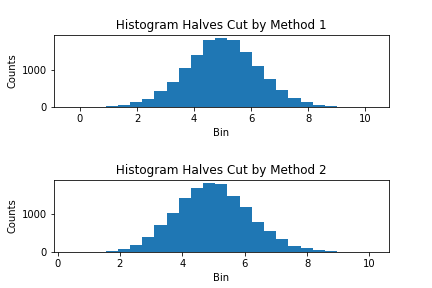
\includegraphics[width=1\linewidth,height=0.5\textheight]{Fig04}
\caption{Histogram of Cut Rods with    Operator's Handling}
\label{fig:Fig04}
\end{figure}

\noindent The yield for method 1 is $49 $\% while for method 2 is $52 $\% respectively.
\end{document}